\documentclass[11pt]{article}
% NAACL 2027 System Demonstrations are single-blind: the [preprint] option keeps author names
% and page numbers. The ACL style files (acl.sty, acl_natbib.bst) are the official ones from
% https://github.com/acl-org/acl-style-files; do not change margins or fonts.
\usepackage[preprint]{acl}
\usepackage{times}
\usepackage{latexsym}
\usepackage{amsmath}
\usepackage[T1]{fontenc}
\usepackage[utf8]{inputenc}
\usepackage{microtype}
\usepackage{inconsolata}
\usepackage{graphicx}
\usepackage{booktabs}
\usepackage{tabularx}
\usepackage{multirow}
\usepackage{float}
\usepackage{tikz}
\usetikzlibrary{arrows.meta,positioning,fit,backgrounds}

\title{Clarify, then Verify: A Payment-Support Assistant That Asks\\Which Record You Mean Before It Answers}

\author{Sandip Nandi \and Apurba Bose \and Aishwarya Bose \and Soovadeep Bakshi \\
  Independent Researchers}

\begin{document}
\maketitle

\begin{abstract}
Customers rarely quote a transaction ID. ``Why was my card declined yesterday?'' can match
several of their payments, and an assistant that guesses which one is meant can give a
correct-sounding answer about the wrong money. We present Finbot, an open-source
payment-support demonstration that joins two steps in one conversation. First, it keeps a
probability for each of the customer's authorized records and asks the one or two short
questions with the highest expected value, then shows a short list for the customer to
confirm; a probability never selects a record on its own. Second, it answers about the
confirmed record only through a gate that checks every amount, status and cause against that
record, with one repair, then an answer built from the record, then refusal. An inspector shows
beliefs, question scores, evidence and every rejected draft. On 224 real Banking77 questions
with the reference removed, answered by simulated customers played by two model families,
one question chosen by expected decision value lifts the share of episodes whose most likely
record is the right one from 13\% to 69--74\% among eight records, while a fixed-order question
reaches 19\%. Requiring
confirmation keeps wrong-record selections at 2--4\%, against 21--26\% if the system acted on
its top guess. Falling back to the full list only when a customer rejects the short list
resolves as many episodes as showing all eight at once, while 51--70\% of customers never scan
eight records. When every candidate has the same amount, one question still puts the right record
first in 46\% of episodes, against 16\% in fixed order. On held-out template drafts the answer
checks reject 82\% of injected errors; with a live Llama 3.3 70B writer, one repair removes an
injected fee in 127 of 128 answers.
\end{abstract}

\section{Introduction}

A payment-support assistant that answers from retrieved records can still be wrong about the
customer's money in two ways. It can state a fact the record does not support, or it can state
a supported fact about the wrong record. The first failure has drawn most of the attention in
grounding and verification work \citep{gao-etal-2023-rarr}. The second begins earlier, when
the customer does not say which payment they mean. ``I was charged twice at the restaurant''
gives no reference; the customer's account may hold five card payments that week.

The usual responses to this are to ask for the reference, which customers often do not have
at hand, or to show the whole list. The first stalls the conversation; the second works when
the customer can read a list, but is long on a phone screen and does not fit a voice channel. Clarifying questions are a well-studied alternative
\citep{rao-daume-iii-2018-learning,aliannejadi2019asking,kuhn2022clam}, and Bayesian
experimental design gives a principled way to choose them \citep{lindley1956measure}. Recent
work applies expected information gain to eliciting what a user wants from a language model
\citep{piriyakulkij2023active,li2025eliciting}.

Finbot puts the two halves in one conversation (Figure~\ref{fig:architecture}). A clarification
step narrows the customer's authorized records with at most two multiple-choice questions and
ends only when the customer confirms a record. A verification step then answers about that
record, and code decides what may be said. The demonstration makes each decision inspectable.
Each part rests on established techniques; what is new is how they are joined. In this
architecture for conversations about ambiguous structured records, a probability ranks records but
never authorizes an answer, and the customer's confirmation is the only path from the
clarification step to the answering step. Our contributions are:
\begin{itemize}\itemsep0pt
\item An interactive system that joins Bayesian record clarification, explicit confirmation and
  corrections with record-grounded answer verification and an evidence inspector.
\item An ambiguity benchmark of 224 real customer questions with their references removed, each
  paired with two to eight similar records, and a simulated-customer protocol with three personas.
\item An evaluation with two simulator families, safety stress tests, a same-amount slice,
  sensitivity, a language-model question chooser, free-text replies, held-out tests of the answer
  checks and a live-writer run. It needs no human participants.
\end{itemize}
The demonstration is meant for people who build assistants over customers' account data, and
for researchers studying clarification and grounded generation. A hosted copy runs at \url{https://finbot-demo-20852907589.us-central1.run.app}. The
system also runs locally with no model account: \texttt{python -m finbot.demo} serves the same pages. The code, data, results and a 2.5-minute video are at
\url{https://github.com/soovadeep/finbot-demo} (MIT license).

\begin{figure*}[t]
\centering
% Original vector diagram; no external image or font asset is required.
\resizebox{\textwidth}{!}{%
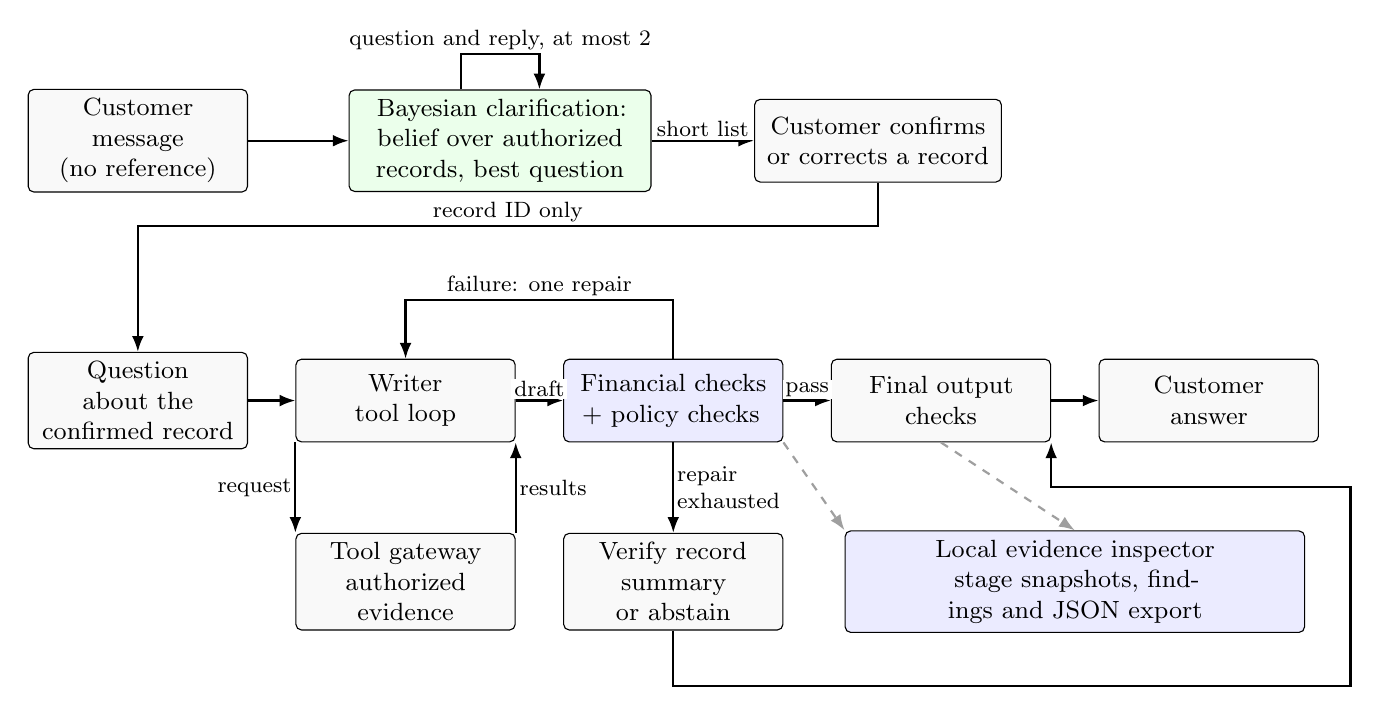
\begin{tikzpicture}[
  box/.style={draw, rounded corners=2pt, align=center, minimum height=1.05cm,
              text width=2.55cm, font=\small, fill=gray!5},
  lab/.style={font=\footnotesize, fill=white, inner sep=1pt},
  arr/.style={-{Latex[length=2mm]}, thick},
  obs/.style={arr, dashed, gray!75}]
% Clarification row
\node[box] (message) at (0,3.3) {Customer message\\(no reference)};
\node[box,fill=green!8,text width=3.6cm,minimum height=1.25cm] (clarify) at (4.6,3.3)
  {Bayesian clarification:\\belief over authorized\\records, best question};
\node[box,text width=2.9cm] (confirm) at (9.4,3.3) {Customer confirms\\or corrects a record};
\draw[arr] (message) -- (clarify);
\draw[arr] (clarify) -- node[above,lab]{short list} (confirm);
\draw[arr] ([xshift=-0.5cm]clarify.north) -- ++(0,0.45) -- node[above,lab]{question and reply, at most 2} ++(1,0) -- ++(0,-0.45);
% Answering row
\node[box] (question) at (0,0) {Question about the\\confirmed record};
\node[box] (writer) at (3.4,0) {Writer\\tool loop};
\node[box,fill=blue!8] (gate) at (6.8,0) {Financial checks\\+ policy checks};
\node[box] (output) at (10.2,0) {Final output\\checks};
\node[box] (answer) at (13.6,0) {Customer\\answer};
\node[box] (evidence) at (3.4,-2.3) {Tool gateway\\authorized evidence};
\node[box] (fallback) at (6.8,-2.3) {Verify record summary\\or abstain};
\node[box,fill=blue!8,text width=5.6cm] (inspector) at (11.9,-2.3)
  {Local evidence inspector\\stage snapshots, findings and JSON export};
\draw[arr] (confirm.south) -- ++(0,-0.55) -| node[pos=0.25,above,lab]{record ID only} (question.north);
\draw[arr] (question) -- (writer);
\draw[arr] (writer) -- node[above,lab]{draft} (gate);
\draw[arr] (gate) -- node[above,lab]{pass} (output);
\draw[arr] (output) -- (answer);
\draw[arr] (gate.north) -- ++(0,0.75) -| node[pos=0.25,above,lab]{failure: one repair} (writer.north);
\draw[arr] (writer.south west) -- node[left,lab]{request} (evidence.north west);
\draw[arr] (evidence.north east) -- node[right,lab]{results} (writer.south east);
\draw[arr] (gate) -- node[right,lab,align=left]{repair\\exhausted} (fallback);
\draw[arr] (fallback.south) -- ++(0,-0.7) -| (15.4,-1.1) -| (output.south east);
\draw[obs] (gate.south east) -- (inspector.north west);
\draw[obs] (output.south) -- (inspector.north);
\end{tikzpicture}%
}

\caption{One conversation in Finbot, in three steps. (1)~Clarification keeps a belief over the
customer's authorized records and asks at most two questions. (2)~The customer confirms one record
from a short list (or none). (3)~Only the confirmed record ID passes to the answering step, where
code controls tool access, the checks and the recovery path, and the model chooses tools and
writes drafts. The inspector observes all three steps (dashed links).}
\label{fig:architecture}
\end{figure*}

\section{System}
\label{sec:system}

\subsection{Clarifying which record}

\paragraph{Candidates and beliefs.}
The session starts from the records the customer is authorized to see; clarification never
retrieves or grants access to anything new. Each candidate has four displayable attributes:
kind (card payment or bank transfer), merchant or payee, date and amount. The belief starts
uniform over up to eight candidates.

\paragraph{Questions and replies.}
Each question $q$ asks for one attribute $k$ and offers the values $O_q$ that distinguish the
remaining candidates, plus ``I'm not sure'' ($?$). Let $h_k$ be candidate $h$'s value. A reply $r$
has likelihood
\[
P(r \mid h, q) = \begin{cases}
u_k & r = {?}\\
(1-u_k)\,a_k & r = h_k\\
(1-u_k)\,\frac{1-a_k}{|O_q|-1} & \text{otherwise,}
\end{cases}
\]
and the belief updates by Bayes' rule, $b'(h) \propto b(h)\,P(r \mid h, q)$, so ``not sure''
carries no information. The settings $(a_k, u_k)$ are $(0.9, 0.1)$ for the kind of payment,
$(0.85, 0.15)$ for the date and $(0.8, 0.2)$ for the payee and the amount. A detail volunteered
in free text enters the same way, with $a = 0.65$ if it is hedged (``I think it was a
transfer''). These are design settings, not measured human accuracy;
Sections~\ref{sec:more} and~\ref{sec:safety} test what happens when they are wrong.

\paragraph{Choosing the next question.}
Three selectors are implemented. \emph{Fixed} asks attributes in a set order.
\emph{Information gain} maximizes $\mathrm{IG}(q) = H(b) - \sum_r P(r)\,H(b_r)$, where $b_r$ is
the belief after reply $r$ and $P(r) = \sum_h b(h)\,P(r \mid h, q)$. With
$e(b) = 1 - \max_h b(h)$, the chance of picking the wrong record, \emph{decision value}
maximizes its expected drop minus a cost $c = 0.02$ per question:
\[
\mathrm{DV}(q) = e(b) - \textstyle\sum_r P(r)\, e(b_r) - c,
\]
and stops when no question has $\mathrm{DV}(q) > 0$. Information gain rewards any reduction of
uncertainty, including among records that are already unlikely; decision value counts only the
drop in the chance of picking the wrong record, the error confirmation guards against, and its
cost lets it stop when another question would barely change that chance. All selectors stop after the budget (two by
default) or once one record holds 95\% of the belief. The live demonstration asks by decision
value, the selector that does best in Section~\ref{sec:eval}, and its inspector shows both
scores.

\paragraph{Confirmation and corrections.}
The customer then sees the most likely records, most likely first, and picks one or says none
match. A high probability is used only to order this list; it never selects a record. The
customer can change the selection later. A correction increases a revision counter and
discards the earlier answer, so no answer about the old record survives.

\subsection{Answering about the confirmed record}

The confirmed record ID is the only thing that passes to the answering step, which fetches the
record again through a gateway scoped to the customer's session. A model drafts the answer in a
tool loop. Before anything is shown, deterministic checks compare every amount, currency, date,
status, cause and reason code in the draft with the record and with the policy table; they also
check that the returned record carries the requested ID. A failing draft gets one repair; if
that fails too, code builds an answer from the record and checks it; refusal comes last. Fields
written by third parties, such as merchant descriptors, are shown to the model but cannot vouch
for a stated fact.

\paragraph{Security boundaries.} The customer's tenant comes from the authenticated session, and
the tool schemas have no tenant field, so the model cannot widen its scope. The confirmed ID is
held by code, not by the model, and the confirmed record is the only one the answering step can
read: a lookup of any other ID, including the customer's other candidates, returns ``not found'',
so no other record can become evidence. A lookup that returns a record other than the one requested
is rejected, as is an ID in the draft that was not looked up. Third-party text and log messages are
never evidence.

The checks are deterministic extractors, not a model. Regular expressions and small phrase
tables pull out of the draft every money amount and currency, date, card's last four digits,
reason code and URL, and every status or cause stated in words (``it was declined because the
card was reported lost''), with negation and hedges handled. Each extracted value must occur in
the tool results for the confirmed record and the session's tenant, and a cause in words must
map to the recorded reason code; otherwise the draft is rejected with a reason such as
\texttt{ungrounded\_amount:12.34}. A policy statement must reproduce a sentence of the help page
it cites. A companion paper evaluates these checks at scale and is not needed here: this paper
contributes the clarification step, the confirmation that joins it to the checks, and the
inspector that shows both.

\subsection{What the inspector shows}

The demonstration page holds the conversation on the left and an inspector on the right. During
clarification the inspector shows the belief over candidates as bars and, for every question
it considered, the expected information gain and how much the question would cut the chance of
picking the wrong record, so a reviewer can see why a question was chosen. Details the
customer volunteers in free text, including hedged ones (``I think it was a transfer''), are
parsed with small visible rules and enter the belief as weaker evidence. After confirmation it shows the retrieved record and a numbered account
of how the answer was checked: which records were fetched, each rejected draft with its reasons
in plain words and the rejected text, and whether the final answer is the model's own, a repair
or built by code. An ``injected model fault'' menu adds a wrong status, a wrong amount once,
a wrong amount every time, or no fault, so a reviewer can watch each recovery path.

\paragraph{Writers.} By default the hosted page and \texttt{python -m finbot.demo} draft answers
with a scripted writer over synthetic records, so reviewers need no key and every run is
reproducible; clarification itself uses no language model. A switch on the hosted page has a live
model (Llama 3.3 70B through OpenRouter) write the answer about the confirmed record instead, inside
the same conversation and behind the same checks, repair and fallback; the fault menu applies to
either writer. Live answers are capped per visitor and per day, and the scripted writer answers
when the cap is reached or the provider fails. The command-line assistant
(\texttt{python -m finbot.app}) runs the same checks around any configured model, including local
Ollama models, but expects a reference.

\section{Demonstration walkthrough}

\begin{figure*}[t]
\centering
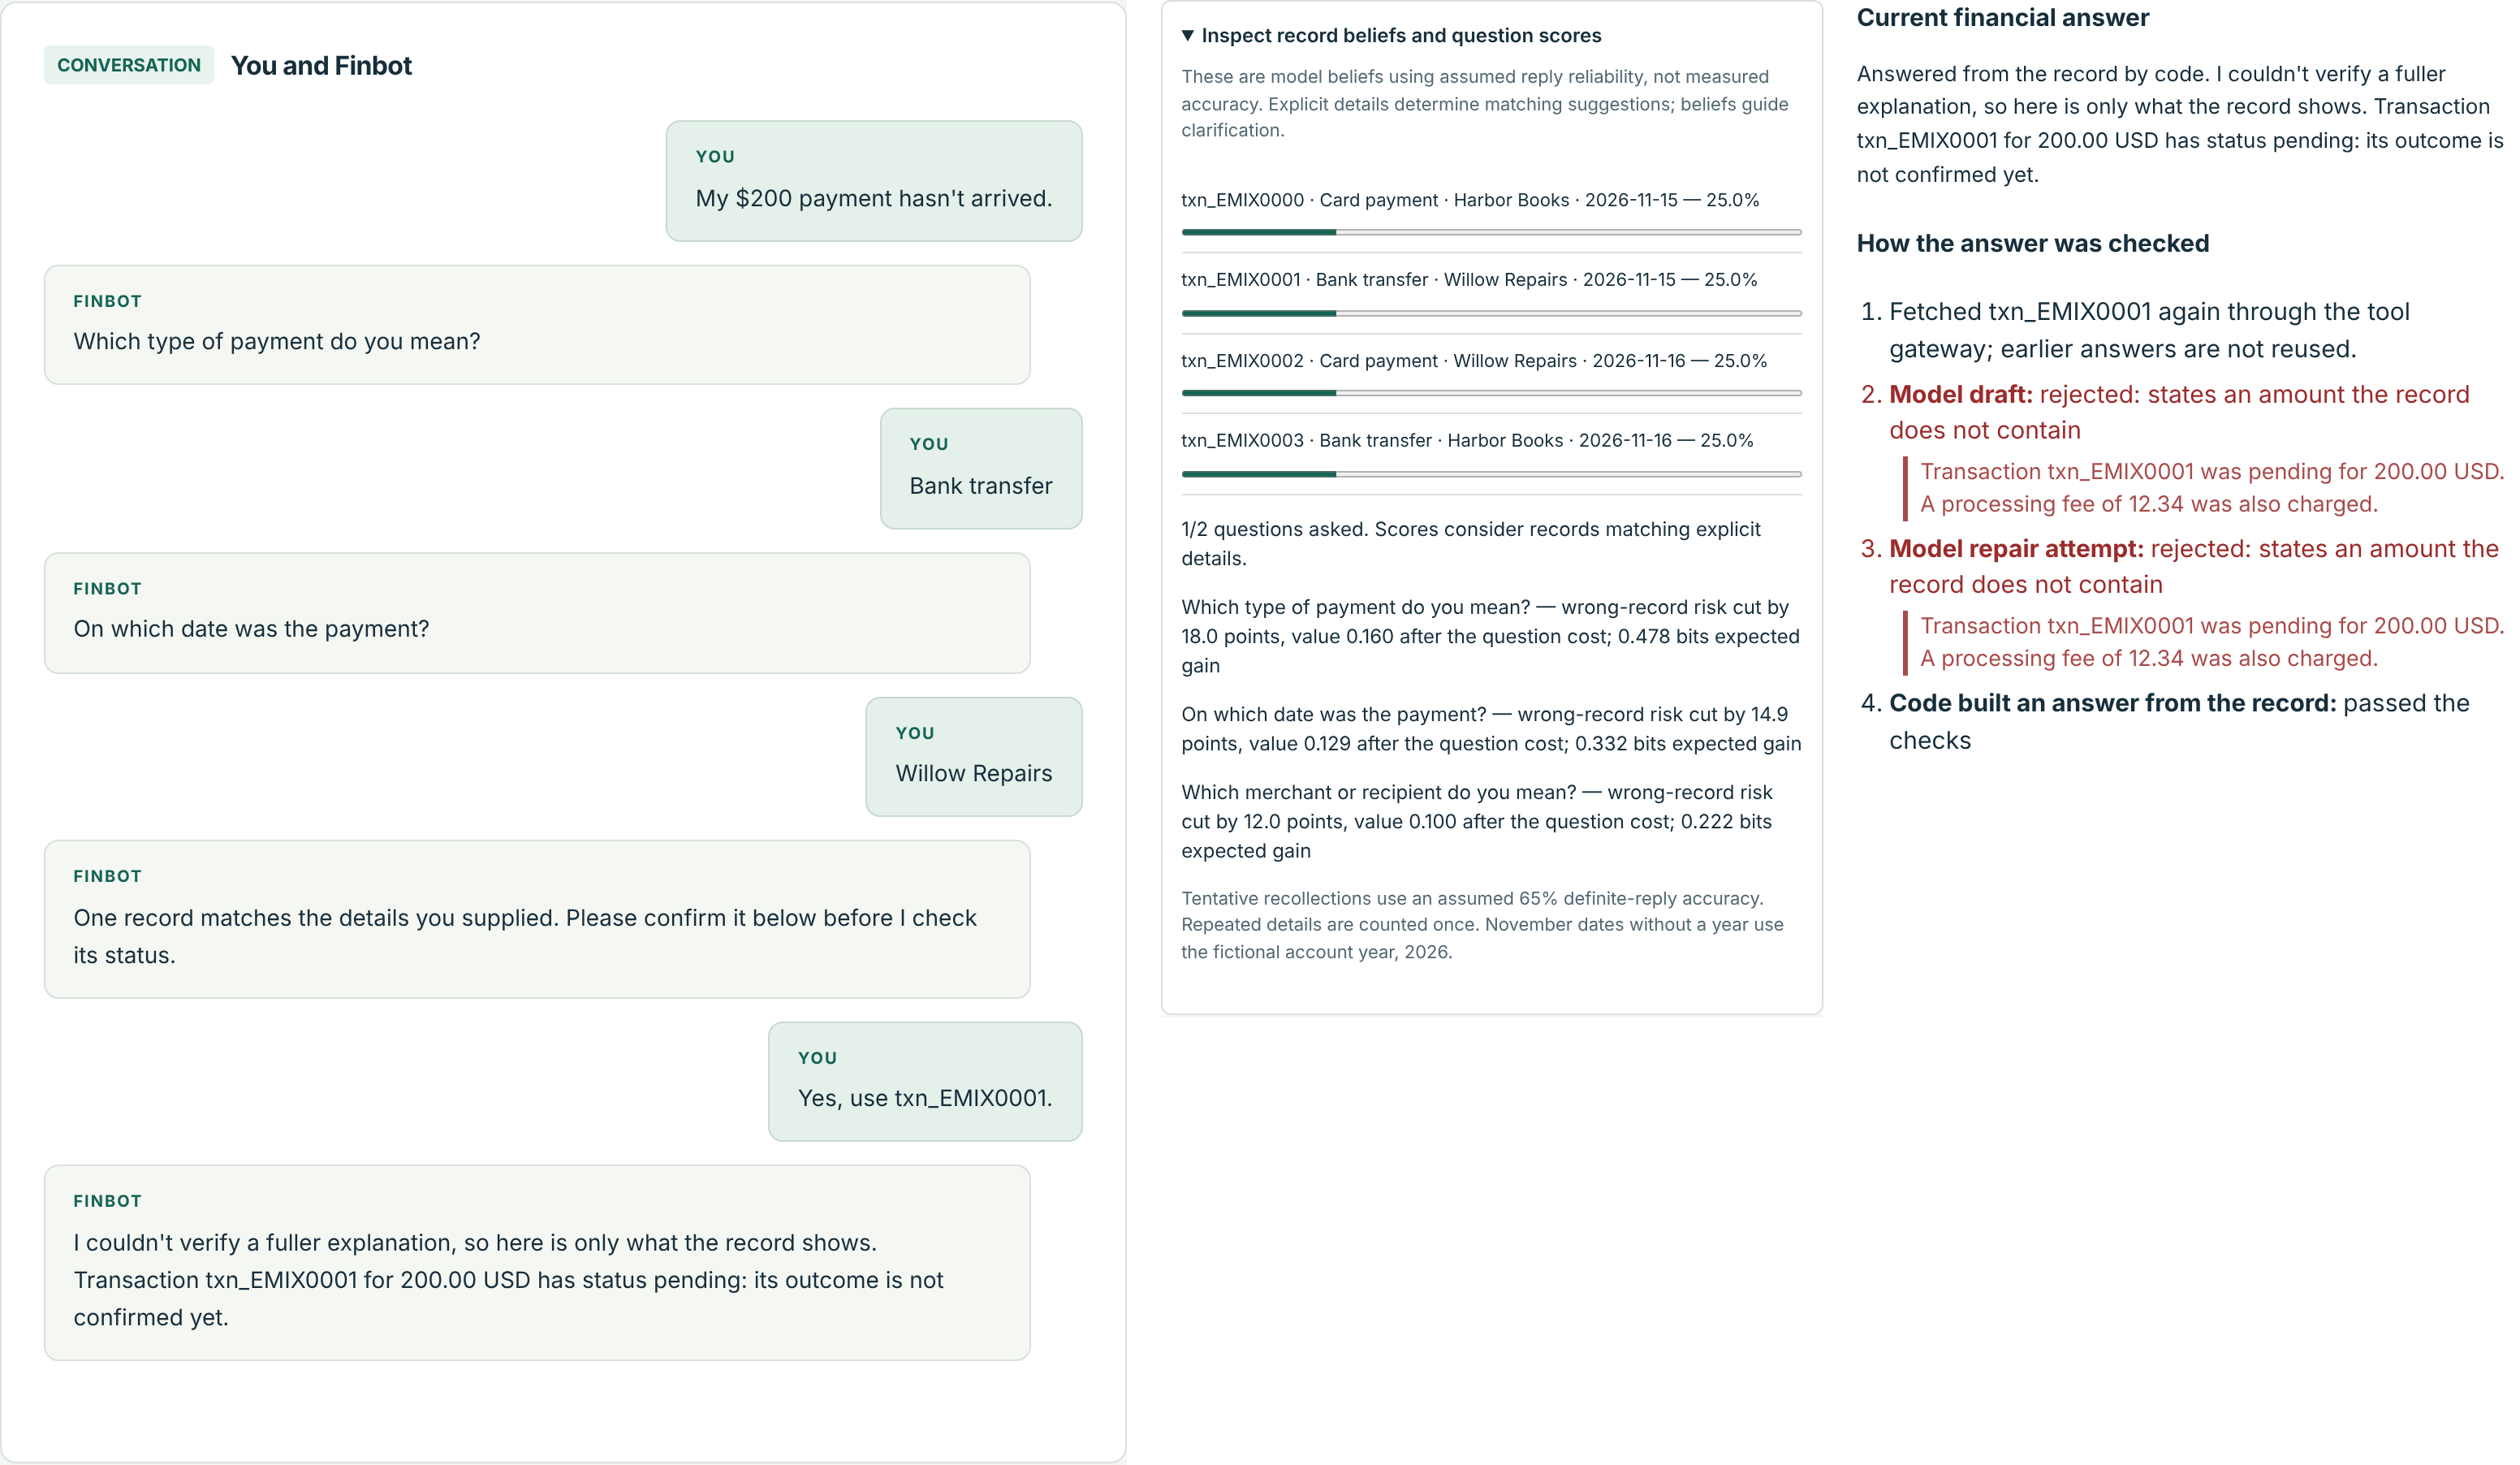
\includegraphics[width=\textwidth]{conversation.png}
\caption{The walkthrough in the hosted demo, with the fault menu set to ``wrong amount every
time''. (a)~Two questions narrow four \$200 payments to one, which the customer confirms.
(b)~The belief inspector at the first question: four records at 25\% each, and each question's
decision value and information gain. (c)~The check of the answer: the record is fetched again,
the draft and its repair are rejected for stating a fee the record does not contain, and code
builds the answer from the record.}
\label{fig:screenshot}
\end{figure*}


Figure~\ref{fig:screenshot} shows this conversation. The account holds four \$200 payments: a
card payment and a bank transfer to each of two payees, on November 15 and 16. The customer writes
``My \$200 payment hasn't arrived.'' The amount rules nothing out, and each remaining question
splits the records in half, so payment type (0.48 bits), date (0.33) and payee (0.22) differ only
through their reliabilities. The customer says it was a bank transfer and, asked for the date,
replies ``Willow Repairs'', which the parser takes as the payee. One record now holds 72\% of the
belief and is offered for confirmation, with the others still listed. With the fault menu at
``wrong amount every time'', the draft and its repair both add a 12.34 fee and are rejected
(\texttt{ungrounded\_amount:12.34}), and the customer sees an answer built from the record: the
200.00 USD transfer is pending. If the customer then writes ``Actually, it was a card payment on
November 16'', that answer is discarded and the matching card record is offered.

\begin{table}[t]
\centering\small
\footnotesize
\setlength{\tabcolsep}{2.2pt}
\begin{tabular}{@{}lcccc@{\hspace{5pt}}ccc@{}}
\toprule
 & & \multicolumn{3}{c}{Haiku 5.5} & \multicolumn{3}{c}{Llama 3.3 70B} \\
\cmidrule(lr){3-5}\cmidrule(l){6-8}
Strategy & Qs & Top-1 & Corr. & Wr. & Top-1 & Corr. & Wr. \\
\midrule
None & 0 & 13 & 17 & 3.1 & 13 & 21 & 5.4 \\
Fixed, 1 & 1 & 19 & 24 & 2.2 & 19 & 30 & 5.8 \\
IG, 1 & 1 & 65 & 44 & 2.2 & 70 & 59 & 4.0 \\
DV, 1 & 1 & 69 & 47 & 2.2 & 74 & 63 & 4.0 \\
Fixed, 2 & 1.95 & 72 & 48 & 1.8 & 77 & 66 & 4.0 \\
IG, 2 & 1.95 & 73 & 46 & 1.8 & 78 & 66 & 4.0 \\
DV, 2 & 1.36 & 74 & 49 & 2.2 & 79 & 66 & 4.0 \\
\quad + fallback & 1.36 & n/a & 66 & 3.1 & n/a & 81 & 4.9 \\
Show all 8 & 0 & n/a & 60 & 1.8 & n/a & 81 & 3.6 \\
\bottomrule
\end{tabular}
\caption{Eight candidate records, 224 episodes, mixed personas (\%). Fixed: fixed order; IG: information gain; DV: decision value; the number is the question
budget; None shows the first two records. Qs: mean questions asked with Haiku customers (Llama: 1.31 for DV, 2). Top-1: episodes whose most likely record
after the questions is the target. Corr.\ and Wr.: episodes in which the customer
confirmed the target or another record from the two-record short list (or from all eight).
``+ fallback'' shows all eight only to customers who reject the short list. Correct-rate
intervals are about $\pm$6 points.}
\label{tab:main}
\end{table}

\section{Evaluation}
\label{sec:eval}

\subsection{Ambiguity benchmark}

We take every Banking77 test question \citep{casanueva-etal-2020-efficient} in our two
evaluation sets that is backed by a card payment or a bank transfer, 224 in all, and delete the
transaction or transfer reference from the text with rules (``Re txn\_\ldots:'' and bracketed IDs
are removed; a bare ID becomes ``it''). The original record is the hidden target. It is joined
by similar records from the same customer: the same kind of payment where possible, then the
nearest dates, with ties broken at random (seed 2027). The questions are real customer wording;
the records come from a seeded synthetic generator: each customer pays a few invented merchants
and payees (a transfer's payee is an account such as ``account ending 6811''), dates fall in
October and November 2026, and no two records in an episode share an amount. The main set fixes
eight candidates per episode; a target shares its kind with 6.6 of the seven others on average,
its payee with 4.0 and its date with 2.2. A second set draws two to five (mean 3.6). In 153 of the
224 episodes a distractor has the same kind and date as the target. In 192 episodes the question
is \emph{naturally fitting}: what it asks about is consistent with its record (criteria in
Appendix~\ref{app:bench}). Results on these 192 differ from those on all 224 by at most three
points. Because amounts are unique, an answer about the amount identifies a record outright;
Section~\ref{sec:same} removes this shortcut.

\subsection{Simulated customers}

A language model plays the customer. It sees its opening message and a memory note, never the
candidate list until the confirmation step, and it answers in JSON. Each episode gets one of three
personas, assigned by a fixed seed: \emph{receipt} (40\%) knows every detail; \emph{vague}
(35\%) remembers the payee and month and a rounded amount; \emph{misremembers} (25\%) is
confident about one wrong detail taken from another candidate. Unlike the demonstration, the
simulated customer answers only through the question's options. The system prompt tells the
model to say it is not sure whenever its note does not settle a question. We run two model
families, Claude Haiku 5.5 and Llama 3.3 70B Instruct, so that results do not rest on one
simulator. Replies are cached per question and per list, so every selector meets the same
customer and differences between selectors come from the questions they ask. The study made
9,501 model calls and cost under US\$5.

We compare five strategies: no questions (show the first two records), the three selectors,
and the reference baseline of showing every candidate at once. An episode is \emph{correct}
when the customer confirms the target, \emph{wrong} when they confirm another record, and
\emph{unresolved} when they pick none. All intervals are 95\% Wilson intervals.



\paragraph{Results.}
Table~\ref{tab:main} gives the main results. Among eight records, one Bayesian question puts
the target first in 65--74\% of episodes, against 19\% for a question asked in fixed order and
13\% for none; the customer then confirms the target in 44--63\% of episodes, about twice the
fixed-order rate under both simulators. With a budget of two, fixed order catches up (48\% and
66\% correct) but asks 1.95 questions; decision value reaches the same rates with 1.31 to
1.36, because it stops when another question is not worth asking. On the smaller set (two to five records), the selectors differ
little: one question in any order already puts the target first in 64--70\% of episodes.

Showing every record at once resolves more episodes than the short list alone (60\% and 81\%):
the simulated customers are good at scanning lists. The two combine well: when the customer
rejects the short list, the system shows the full list. Decision value followed by this fallback confirms the target in
66\% (Haiku) and 81\% (Llama) of episodes, matching or beating the full list, while only 49\%
and 30\% of customers ever see eight records; wrong selections rise slightly, to 3.1\% and
4.9\%, because a customer gets two chances to choose. Where a long list
cannot be shown at all, as in voice, the questions alone reach about 80\% of the full-list
success. The simulators differ mainly on vague customers, whom Haiku often leaves unresolved,
as its prompt asks (Appendix~\ref{app:bench}).

\paragraph{Without unique amounts.}
\label{sec:same}
Decision value asks for the amount first in 128 of 224 episodes (fixed order: 11). A second copy
of the set gives every candidate the target's amount and currency; only 99 targets then differ
from all others in kind, payee or date. One decision-value question puts the target first in 46\%
of episodes (fixed order 16\%, none 13\%) and in 85\% of the 99 (fixed order 18\%). On those 99,
decision value with two questions confirms the target in 68\% (Haiku) and 85\% (Llama) with
2--3\% wrong, against 73\% and 88\% for the full list. In the other 125 the target has a twin that
no question or list can separate, and wrong picks match the full list's (Appendix~\ref{app:same}).

\subsection{Sensitivity, baseline and free text}
\label{sec:more}

Three further studies reuse the cached replies (eight records, budget two;
Appendix~\ref{app:studies}). Within this benchmark, one reliability for every attribute, from 0.6
to 0.99, changes no question: the amount question then always scores highest, and after its
answer no single question can change the most likely record, so decision value stops. Twenty
random draws of the four reliabilities move correct confirmations by at most nine points. Claude
Sonnet 5.5 choosing the questions reaches 43\% and 63\% correct, against 49\% and 66\%. With
free-text replies, the rules read 63\% of definite answers with one wrong read in 670 replies, and
correct confirmations fall to 42\% and 51\%.

\subsection{Safety under wrong assumptions}
\label{sec:safety}

Acting on the top guess after the questions would pick the wrong record in 26\% (Haiku) and
21\% (Llama) of episodes; with confirmation, wrong selections are 2.2\% (0.9--5.1\%) and 4.0\%
(2.1--7.5\%), no higher than showing the whole list (1.8\% and 3.6\%). When every customer is
confident about one wrong detail, acting on the top guess would be wrong in 42\% of episodes, while
confirmation keeps wrong selections at 5.4\% and 5.8\%, in line with the full list (4.5\% and
7.6\%); the rest confirm the record their mistaken memory matches. If the system assumes every
reply is right 99\% of the time, it stops sooner on the smaller set and wrong selections are
unchanged (4.9\% and 5.8\%): a wrong belief only reorders the short list.

\subsection{Answer checks}
\label{sec:inject}

\paragraph{Template tests.} In controlled claim-level tests (no model), we write for each of the
224 target records five correct drafts and 14 or 15 drafts with one injected error, and check each
with the stored record as the only evidence. A first run caught 96\% of 3,270 errors but 81\% of
wrong statuses; after we added the missing paraphrases (``went through'', a bare ``failed''), the
same drafts give 98.9\%. Because that number is tuned, a held-out set with new frames and wordings
was run once, unchanged: the checks reject 82\% of 3,240 errors (all amounts, fees, currencies and
IDs and 92\% of statuses, but few numeric dates, letter-prefixed codes and bare \texttt{www}
links) and 10\% of 1,120 correct drafts, all ``has not settled yet'' about a pending transfer,
which the gate then answers from the record (Appendix~\ref{app:inject}).

\paragraph{A live writer.} With Llama 3.3 70B answering about each of the 128 card-payment
targets, 125 first drafts pass; the other three are false rejections (``American Express'' for
\texttt{amex}, a channel value read as an ID), recovered by repair or the record-built answer. One
repair removes a fee injected into the first draft in 127 of 128 answers; injected into the repair
too, all 128 end in the record-built answer. Passing drafts were not checked by hand. Interface and
accessibility checks are in Appendix~\ref{app:iface}.

\section{Related work}

Clarifying questions have been ranked by expected usefulness \citep{rao-daume-iii-2018-learning},
asked in open-domain search \citep{aliannejadi2019asking,zhang2020evaluating}, asked selectively
when a request is ambiguous \citep{kuhn2022clam}, and chosen by expected information gain to
elicit what a user wants from a language model \citep{piriyakulkij2023active,li2025eliciting}.
Simulated users can evaluate such systems before human studies \citep{sekulic2022evaluating}. In Finbot the hypotheses are the customer's own authorized records,
the options come from those records, and the stopping rule targets the chance of naming the wrong
one. Post-hoc revision against evidence \citep{gao-etal-2023-rarr}, programmable rails
\citep{rebedea-etal-2023-nemo} and capability-based separation of control and data
\citep{debenedetti2025camel} motivate the answering step; none picks the record.

\section{Limitations}

The customers are language models, not people: they read lists well, follow persona notes more
consistently than people do, and may share blind spots across the two families, so the results
describe the simulated setting, and the personas' shares are chosen. The records are synthetic, the
Banking77 questions were not written about them (32 are not naturally fitting), the reliabilities
are chosen, not fitted, and the main set's unique amounts favour the amount question. Candidates
are capped at eight; larger accounts need a first filter. The answer checks are English rules over
a fixed set of claim types, and claims outside their vocabulary pass, as 18\% of held-out injected
errors did; the live-writer run covers one model, and no passing draft was checked by hand. The
free-text rules miss common ways of naming payees and dates, and corrections are tested only by
scripted checks. No human or voice evaluation has been done. Finbot is a research demonstration,
not a system validated for production financial support.

\section*{Ethics and broader impact}

Telling a customer the wrong thing about their money can cost them fees, repeated charges or
missed disputes. The design choice we evaluate, that a probability never selects a record, trades
some resolved conversations for fewer answers about the wrong payment, and we report both sides.
The demonstration uses synthetic records and executes no payments. Simulated customers were used
so that no person's financial data was needed; a deployment would need its own consent, retention
and access controls.

\section*{Acknowledgements}

The authors used AI assistants during this project. Anthropic's Claude Code helped write code,
run the evaluations and draft and edit this paper, and OpenAI Codex helped with earlier
implementation and documentation. Claude Haiku 5.5 and Llama 3.3 70B Instruct played the
simulated customers. The authors reviewed and take responsibility for all content, code and
results.

\bibliography{references}

\appendix
\raggedbottom

\section{Reproducibility}
\label{app:repro}

\paragraph{Models.} Simulated customers: \texttt{claude-haiku-5-5} through the Anthropic API
(default sampling, at most 200 output tokens, no extended thinking) and
\texttt{meta-llama/llama-3.3-70b-instruct} through OpenRouter (temperature 0, at most 80 output
tokens). Question chooser (Section~\ref{sec:more}): \texttt{claude-sonnet-5-5} (default sampling,
no extended thinking). Live writer (Section~\ref{sec:inject} and the hosted switch): the same Llama
model through OpenRouter (default sampling, at most 400 output tokens). The clarification step
itself and the answer checks use no model.

\paragraph{Seeds and caches.} The benchmark is built with seed 2027
(\url{scripts/naacl2027/build_ambiguity_set.py}); each episode's persona and misremembered
detail are drawn from seeds derived from the episode ID, so every selector and simulator meets the
same customer. The injected-error test and the 20 reliability draws also use seed 2027. Every
simulator reply is cached on disk with the prompt that produced it
(\url{results/naacl2027/clarification-sim/cache-*.jsonl} and
\url{results/naacl2027/review-studies/}), so the tables can be recomputed without model calls.

\paragraph{Scripts.} \texttt{simulate\_customers.py} (main study), \texttt{review\_studies.py}
(Section~\ref{sec:more}), \texttt{build\_same\_amount\_set.py} (Section~\ref{sec:same}),
\texttt{check\_injection.py} and \texttt{live\_writer\_run.py} (Section~\ref{sec:inject}), all in
\texttt{scripts/naacl2027/}. Intervals are 95\% Wilson score intervals ($z = 1.96$). The
follow-up studies made about 3,500 further model calls and cost under US\$5.

\section{Simulator prompts}
\label{app:prompts}

\paragraph{System prompt.} \emph{You are role-playing a bank customer in a support chat, for a
software test. Stay in character. Use only what your memory note says. If the note does not tell
you the answer, say you are not sure. Never invent certainty you do not have. Reply with JSON only,
no other text.}

\paragraph{Memory notes.} Receipt and misremembers (with one detail taken from another
candidate): \emph{You have the details in front of you: a $\langle$kind$\rangle$ to
$\langle$payee$\rangle$ on $\langle$date$\rangle$ for $\langle$amount$\rangle$.} Vague:
\emph{You remember it was a $\langle$kind$\rangle$ to $\langle$payee$\rangle$, some time in
$\langle$month$\rangle$, for roughly $\langle$rounded amount$\rangle$. You do not remember the
exact day or the exact amount.}

\paragraph{Turns.} Each prompt repeats the opening message and the memory note, then gives the
question and its options (reply \texttt{\{"choice": \ldots\}}), the short list or full list
(reply \texttt{\{"number": \ldots\}}, 0 for none), or, in the free-text study, the question alone
(\emph{Answer in your own words, in one short sentence, as a customer would type it in a chat}).
The chooser sees the opening message, every candidate's kind, payee, date and amount, the
questions so far with their answers, and the remaining questions with their options, and replies
\texttt{\{"ask": \ldots\}} or \texttt{\{"ask": "stop"\}}.

\section{Benchmark fit and personas}
\label{app:bench}

\paragraph{Naturally fitting.} A question is naturally fitting when nothing it says contradicts its
record: 32 questions fail this, those whose Banking77 intent concerns an ATM withdrawal or cash
(paired with a card payment) or a pending payment (paired with a record that is not pending). All
other intents (card declines, refunds, transfers, charges and so on) fit any record of the matching
kind. Table~\ref{tab:fit} compares the two sets.

\paragraph{Personas.} The two simulators differ mainly on \emph{vague} customers. Haiku leaves 54\% of them
unresolved even when shown all eight records, against 1\% for Llama: it declines to pick when
its note does not settle the choice, as its prompt asks. With complete receipts, both resolve
most episodes (80\% and 96\% correct with decision value), and both fail on customers who
misremember (8\% and 13\%), who reject short lists that do not match their memory. Vague Haiku
customers resolve more with the fallback than with the full list at once (57\% against 46\%): after
the questions the short list holds fewer records that fit their note, and Haiku declines to choose
among several that do.

\begin{table}[H]
\centering\small
\setlength{\tabcolsep}{3pt}
\resizebox{\columnwidth}{!}{%
\begin{tabular}{@{}lcccc@{}}
\toprule
 & \multicolumn{2}{c}{Haiku 5.5} & \multicolumn{2}{c}{Llama 3.3 70B} \\
\cmidrule(lr){2-3}\cmidrule(l){4-5}
Strategy, measure & All 224 & Fitting 192 & All 224 & Fitting 192 \\
\midrule
No questions, top-1 & 13.4 & 14.1 & 13.4 & 14.1 \\
Fixed order 1, top-1 & 18.8 & 18.2 & 19.2 & 18.8 \\
Decision value 1, top-1 & 69.2 & 68.8 & 74.1 & 74.0 \\
Decision value 2, correct & 48.7 & 51.6 & 66.1 & 67.7 \\
Show all 8, correct & 60.3 & 63.0 & 81.2 & 83.3 \\
\bottomrule
\end{tabular}}
\caption{Each row is one strategy and measure; columns give all 224 episodes and the 192
naturally fitting ones, per simulator (\%).}
\label{tab:fit}
\end{table}

\begin{table}[H]
\centering\small
\setlength{\tabcolsep}{2.5pt}
\resizebox{\columnwidth}{!}{%
\begin{tabular}{@{}llcccc@{}}
\toprule
 & Persona ($n$) & DV1 top-1 & DV2 correct & + fallback C/W/U & All 8 C/W/U \\
\midrule
\multicolumn{6}{@{}l}{\emph{Haiku 5.5 customers}} \\
 & Receipt (89) & 99 & 80 & 98/1/1 & 96/1/3 \\
 & Vague (72) & 43 & 46 & 57/0/43 & 46/0/54 \\
 & Misremembers (63) & 57 & 8 & 30/10/60 & 27/5/68 \\
\midrule
\multicolumn{6}{@{}l}{\emph{Llama 3.3 70B customers}} \\
 & Receipt (89) & 99 & 96 & 100/0/0 & 98/0/2 \\
 & Vague (72) & 58 & 76 & 93/6/1 & 97/1/1 \\
 & Misremembers (63) & 57 & 13 & 40/11/49 & 40/11/49 \\
\bottomrule
\end{tabular}}
\caption{Results by persona, eight records (\%). C/W/U: correct, wrong and unresolved.}
\label{tab:persona}
\end{table}

\section{Sensitivity, chooser and free text}
\label{app:studies}

\paragraph{Reliabilities and question cost.} Within this benchmark, one common reliability for
all attributes, from 0.6 to 0.99, changes no question or outcome. With equal reliabilities the
amount question, whose options split every candidate, scores highest whenever it is offered, and
once it is answered no single further question can change the most likely record, so the one-step
decision value is zero and the selector stops. In 20 draws with each attribute's reliability between 0.6
and 0.99, correct confirmations stay within 40--50\% (Haiku) and 63--67\% (Llama), against 49\% and
66\% by default, and wrong selections within 2.2--2.7\% and 4.0--4.9\%. A question cost from 0 to
0.1 cuts mean questions from about 1.5 to 1.1 and moves correct rates by at most one point.

\paragraph{A language model chooses the question.} Given the message, the candidates and the
same questions, Claude Sonnet 5.5 asks a question or stops; the belief update and short list are
unchanged. It reaches 43\% (Haiku) and 63\% (Llama) correct, against 49\% and 66\% for decision
value, with equal wrong rates. It mostly asks for the amount, which identifies a record exactly
but is what vague customers remember least.

\paragraph{Free-text replies.} When the simulated customer answers in its own words, the
demonstration's rules read 300 of the 475 replies whose option answer was definite (63\% coverage)
and none wrongly; they abstain on the other 175, mostly payees given as account digits, day-first
dates and approximate amounts. Of 195 replies whose option answer was ``not sure'', they read a
value from one (1 wrong read in 670).
Correct confirmations fall to 42\% and 51\%; wrong selections stay at 2.2\% and 4.9\%.

\begin{table}[H]
\centering\small
\setlength{\tabcolsep}{2.6pt}
\resizebox{\columnwidth}{!}{%
\begin{tabular}{@{}llcccc@{}}
\toprule
& Setting & Qs & Top-1 & Correct & Wrong \\
\midrule
\multicolumn{6}{@{}l}{\emph{Haiku 5.5 customers}} \\
 & Default ($c = 0.02$) & 1.36 & 73.7 & 48.7 & 2.2 \\
 & One reliability, 0.6--0.99 & 1.21 & 73.2 & 49.6 & 2.2 \\
 & 20 random draws & 1.17--1.75 & n/a & 40--50 & 2.2--2.7 \\
 & $c = 0$ / $c = 0.1$ & 1.50 / 1.17 & 72.8 / 73.2 & 49.1 / 49.6 & 2.7 / 2.2 \\
 & Sonnet 5.5 chooses & 1.29 & 62.9 & 42.9 & 2.2 \\
 & Free-text replies & 1.51 & 62.1 & 42.0 & 2.2 \\
\midrule
\multicolumn{6}{@{}l}{\emph{Llama 3.3 70B customers}} \\
 & Default ($c = 0.02$) & 1.31 & 78.6 & 66.1 & 4.0 \\
 & One reliability, 0.6--0.99 & 1.16 & 78.1 & 66.1 & 4.0 \\
 & 20 random draws & 1.11--1.75 & n/a & 63--67 & 4.0--4.9 \\
 & $c = 0$ / $c = 0.1$ & 1.45 / 1.12 & 77.7 / 78.1 & 66.1 / 66.1 & 4.0 / 4.0 \\
 & Sonnet 5.5 chooses & 1.18 & 74.1 & 62.9 & 4.0 \\
 & Free-text replies & 1.48 & 61.6 & 50.9 & 4.9 \\
\bottomrule
\end{tabular}}
\caption{Decision value with a budget of two, eight records, mixed personas (\%). ``One
reliability'' sets every attribute's $a_k$ to the same value; every value from 0.6 to 0.99 gives
the same row. Random draws set each $a_k$ independently between 0.6 and 0.99.}
\label{tab:studies}
\end{table}

\section{Interface checks}
\label{app:iface}

An automated Chromium walkthrough runs 18 acceptance checks on the inspector, including every
preset scenario, trace export, keyboard navigation, stale inputs and layouts from 320 to 1440
pixels wide; all 18 pass. A second script exercises the conversation page: parsing the
customer's message, questions, unknown replies, corrections, an unmatched payment and the mobile
layout. axe-core 4.10.3 finds no WCAG 2.1 A or AA violations in 14 interface states (ten of the
inspector, four of the conversation, including a fault-injected answer), with color contrast
left for manual review where it could not be computed. No page made an external request or
raised a script error. These are feature checks, not measures of user comprehension.

\section{Same-amount slice}
\label{app:same}

\begin{table}[H]
\centering\small
\setlength{\tabcolsep}{3pt}
\resizebox{\columnwidth}{!}{%
\begin{tabular}{@{}lcccccc@{}}
\toprule
 & \multicolumn{2}{c}{Top-1} & \multicolumn{2}{c}{Haiku C/W} & \multicolumn{2}{c}{Llama C/W} \\
\cmidrule(lr){2-3}\cmidrule(lr){4-5}\cmidrule(l){6-7}
Strategy & All & Ident. & All & Ident. & All & Ident. \\
\midrule
No questions & 13.4 & 16.2 & 12/15 & 20/2 & 17/29 & 24/2 \\
Fixed order, 1 & 16.1 & 18.2 & 14/8 & 24/3 & 22/31 & 28/2 \\
Info.\ gain, 1 & 39.3 & 70.7 & 28/8 & 56/2 & 39/31 & 68/2 \\
Decision value, 1 & 45.5 & 84.8 & 30/8 & 61/2 & 43/31 & 77/2 \\
Fixed order, 2 & 49.1 & 92.9 & 31/8 & 63/3 & 47/31 & 85/2 \\
Decision value, 2 & 47.3 & 88.9 & 33/8 & 68/3 & 47/31 & 85/2 \\
Show all 8 & n/a & n/a & 35/7 & 73/0 & 50/32 & 88/2 \\
\bottomrule
\end{tabular}}
\caption{Eight records that all share the target's amount and currency (\%). All: 224 episodes.
Ident.: the 99 whose target differs from every other candidate in kind, payee or date. Top-1 is
from Haiku's replies (Llama's differ by at most one point). C/W: correct and wrong confirmations.
Decision value asks the date first in 147 episodes and the payee in 66; fixed order asks the date
in 117 and the kind in 96.}
\label{tab:same}
\end{table}

\section{Answer checks by claim type}
\label{app:inject}

\begin{table}[H]
\centering\small
\setlength{\tabcolsep}{4pt}
\resizebox{\columnwidth}{!}{%
\begin{tabular}{@{}lrrrr@{}}
\toprule
 & \multicolumn{2}{c}{Development} & \multicolumn{2}{c}{Held-out} \\
\cmidrule(lr){2-3}\cmidrule(l){4-5}
Injected error & Drafts & Rejected & Drafts & Rejected \\
\midrule
Wrong amount & 448 & 100 & 448 & 100 \\
Added fee & 448 & 100 & 448 & 100 \\
Wrong currency & 224 & 100 & 224 & 100 \\
Unknown record ID & 224 & 100 & 224 & 100 \\
Wrong status & 582 & 100 & 552 & 92.0 \\
Right and wrong mixed & 448 & 97.8 & 448 & 96.9 \\
Wrong date & 448 & 95.5 & 448 & 55.4 \\
Wrong reason code & 224 & 97.8 & 224 & 42.9 \\
Unlisted link & 224 & 100 & 224 & 17.0 \\
\midrule
All injected & 3,270 & 98.9 & 3,240 & 82.3 \\
Correct drafts & 1,120 & 0.0 & 1,120 & 10.2 \\
\bottomrule
\end{tabular}}
\caption{The demonstration's record checks on template drafts about the 224 target records
(rejected, \%). Development: the drafts the status paraphrases were added for; before that change
wrong statuses were rejected in 81.3\% and all errors in 95.6\%. Held-out: new frames and wordings
written after that change and run once. Held-out misses: dates as 11/12/2026, the code R01, a bare
\texttt{www} link, ``was paid'' (declined) and ``has gone through'' (failed). All 114 false
rejections are ``has not settled yet'' about a pending transfer.}
\label{tab:inject}
\end{table}

\end{document}
